% meta.concepts: 3D moment
% meta.tags: realistic
% acknowledge: Peter Seiler & Luke Melander graciously shared Spring 2019 course material
% source: 2019 P. Seiler AEM2011 HW 4

A researcher is building a mount to experimentally test a motor for an uninhabited aerial vehicle (UAV).
To build the mount she must insert a screw in a plank of wood at point A as shown in the diagram 
below. The plank is secured to the workbench at points C and D by clamps. Each clamp is capable of
providing a force up to 50N tangential to the plank. Assume that the forces provided by the clamps act along
the y-direction.

\begin{enumerate}
  \item The researcher first places the clamps at $d = 20 cm$. She uses a power screw-driver which exerts a clockwise
torque of 30 N-m on the plank. What is the value of the force couple and the corresponding force that
has to be provided by the clamps so that the plank remains in equilibrium?
  \item Will the clamps give way (yield) in this situation? In other words, is the force calculated in (a) greater
than the 50N limit? If so, calculate the minimum value of distance $d$ so that the clamps will not give way.
  \item Would your answers change if she inserts the screw at point B instead of point A. Explain briefly.
\end{enumerate}


\begin{figure}[ht!]
  \centering
  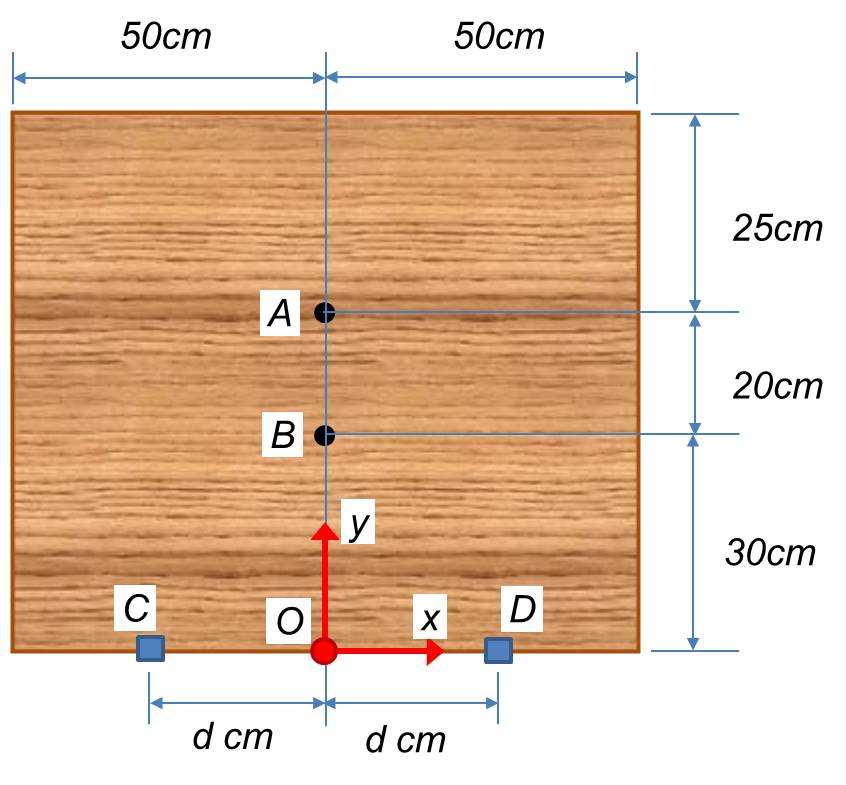
\includegraphics[height=2.0in]{fig.png}
  \caption*{Top-down view of experimental motor mount}
\end{figure}

\iftoggle{flagSoln}{%
\vspace{.5cm}
\rule{\textwidth}{.4pt}
\vspace{.5cm}
\textbf{Solution:}
\begin{figure}[ht!]
  \centering
  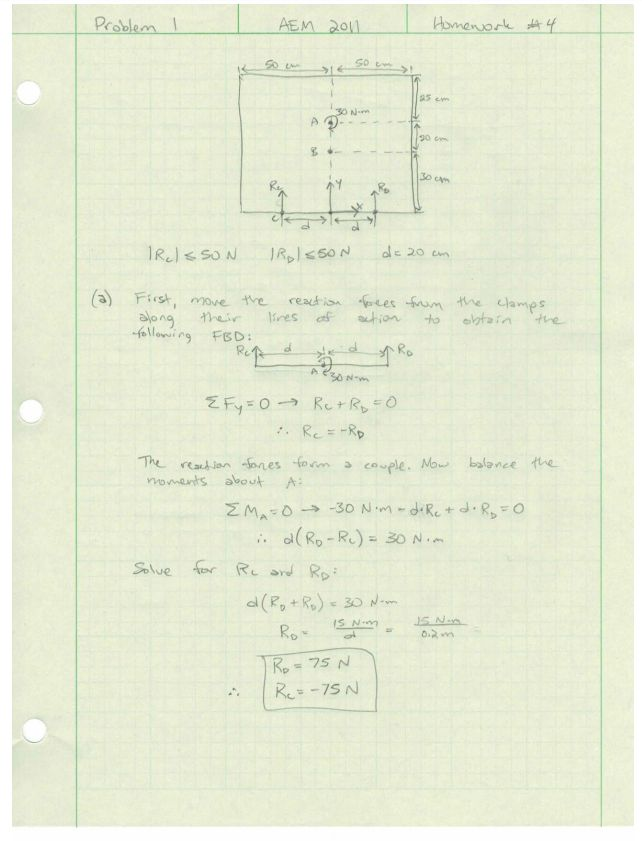
\includegraphics[width=0.45\textwidth,
	           height=0.3\textheight,
		   keepaspectratio]{solna.png}
  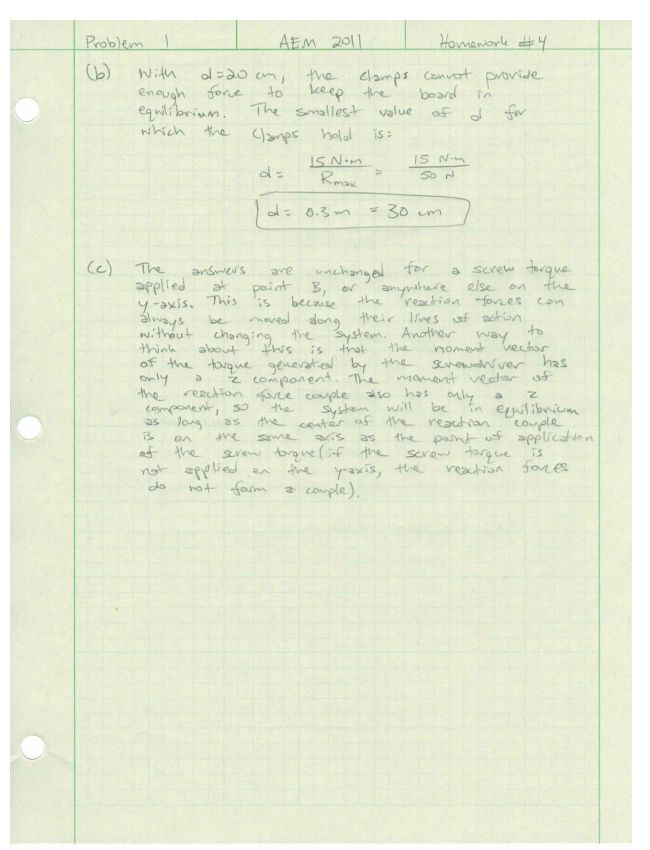
\includegraphics[width=0.45\textwidth,
	           height=0.3\textheight,
		   keepaspectratio]{solnb.png}
\end{figure}
}{%
}%
